\documentclass[sigconf,nonacm,10pt]{acmart}
\settopmatter{printacmref=false, printfolios=false}
\pagestyle{plain}
\usepackage{graphicx}
\usepackage{booktabs}
\usepackage{amsmath}
\usepackage{siunitx}
\usepackage{xeCJK}
\setCJKmainfont{STSong}
\setCJKsansfont{STHeiti}
\setCJKmonofont{STFangsong}
\emergencystretch=3em
\tolerance=1200
\hbadness=10000
\graphicspath{{../figs/}}

\newcommand{\SolEth}{SOL$\to$ETH}
\newcommand{\EthSol}{ETH$\to$SOL}
\newcommand{\Cexec}{C_{\text{exec}}}
\newcommand{\Pnet}{\Pi_{\text{net}}}

\title{第四章 --- Solana $\leftrightarrow$ Ethereum 跨链套利的端到端实证}
\author{匿名}
\affiliation{\institution{-}\country{-}}

\begin{document}
\maketitle

% ══════════════════════════════════════════════════════════════════════════════
\section{Solana $\leftrightarrow$ Ethereum 跨链桥概览}
\label{sec:bridges}
% ══════════════════════════════════════════════════════════════════════════════

当前在 Solana 与 Ethereum 生态之间持续运行、且支持通用资产转移的主流跨链
桥共有五条：Wormhole Portal、LayerZero V2、Mayan Finance、Relay 与
Chainlink CCIP。它们在信任模型、费用结构与验证机制上分别采用不同路线，
由此在延迟、费率与单笔上限上呈现显著差异。
表~\ref{tab:bridges} 汇总其主要参数与我们可以采集到的跨链事件量级。

\begin{table}[h]
  \centering
  \small
  \caption{Solana $\leftrightarrow$ Ethereum 跨链桥对比}
  \label{tab:bridges}
  \begin{tabular}{lllr}
    \toprule
    \textbf{协议} & \textbf{信任/验证} & \textbf{费用模式} & \textbf{记录数} \\
    \midrule
    Wormhole Portal   & Guardian 多签签发 VAA    & 按 gas 计        & 42{,}181 \\
    LayerZero V2      & DVN 验证                 & DVN 费           & 271{,}813 \\
    Mayan Finance     & Dutch auction            & 约 3\,bps        & 10{,}653{,}600 \\
    Relay             & Intent-based fill        & 可变 bps          & 107{,}220 \\
    Chainlink CCIP    & DON + risk manager       & LINK 费          & 2{,}115 \\
    \bottomrule
  \end{tabular}
\end{table}

五条桥中，Wormhole 与 CCIP 采用基于多方证明人的“消息层 + 代币包装”
模型；LayerZero 由 DVN 网络与上层 Oracle/Relayer 分层验证；Mayan 与
Relay 则将跨链结算建模为“订单/拍卖”模式，由 solver 竞价填单。
架构差异直接决定了：（i）跨链事件是否在链上有可核验的 1:1 指纹；
（ii）一次跨链转移能否被单一公开字段精确配对为 (src, dst) 二元组；
（iii）是否存在由中间人定价的“延迟--费用”异质性。
这三点恰好是我们后续能否重建每一次跨链套利 PnL 的关键前提。

% ══════════════════════════════════════════════════════════════════════════════
\section{为何选 Wormhole：数据与套利候选构造}
\label{sec:data}
% ══════════════════════════════════════════════════════════════════════════════

\subsection{为何以 Wormhole Portal 为研究对象}

在前述五条桥中，我们选择 Wormhole Portal 作为唯一的长期样本来源。
原因可归纳为四点：
(i)~\emph{链上可核验}。Portal 的每条消息由 Guardian 集群以密码学签名
背书，并以 VAA（Verifiable Action Approval）形式上链，使我们无需依赖
任何链下台账即可将 Solana 签名与 Ethereum 交易哈希 1:1 配对；
(ii)~\emph{标准化配对}。两链上的 Token Bridge 合约采用固定的
emitter/recipient 字段结构，使 $(arb_{\mathrm{sol}}, arb_{\mathrm{eth}})$
这一“行为者”主键可以直接从链上解码；
(iii)~\emph{传输与执行解耦}。Portal 只完成代币的包装/释放，其后在
目标链上的 DEX 执行是独立的链上事件，使得入场 swap、桥腿、出场 swap
可以分别归因；
(iv)~\emph{代币覆盖最广}。对跨链套利最活跃的长尾 memecoin，Wormhole
通过 WTT 与 NTT 标准所支持的代币集合是其余四条桥的真超集，因此“仅采
Wormhole”不会对套利现象引入显著的样本选择偏差。

\subsection{数据采集流水线}
\label{sec:pipeline}

图~\ref{fig:pipeline} 展示 5 阶段的采集与匹配流水线。
Wormhole 官方的 \texttt{/operations} API 按 VAA 索引，但
\emph{仅保留约 $7$ 天的历史}——不足以支持一年期分析。我们因此
从两条链的 Portal 智能合约\emph{反向出发}：
(1)~分别在 Ethereum 与 Solana 上扫描 Portal Token Bridge 合约的
完整日志/指令，解析出每笔 bridge 事件的 \texttt{src\_chain\_id}
与 \texttt{dst\_chain\_id}；
(2)~以每笔事件的 Solana 签名或 Ethereum 交易哈希作为查询键，
通过 \texttt{wormholescan} 的按签名/哈希搜索接口回溯对应的
VAA（此路径不受 $7$ 天窗口限制）；
(3)~以 VAA（\texttt{emitterChain} $+$ \texttt{sequence}）为外键，
将两链端的签名/哈希合并为统一的跨链记录；
(4)~通过 Birdeye 的 \emph{1~秒级}价格接口查询入场/出场时刻的
代币-USD 汇率；(5)~以贪心配对算法把 bridge 事件前后的同 wallet
swap 归因到本次跨链，形成
(direction, sol\_sig, eth\_hash, entry\_swaps, exit\_swaps,
$\Cexec^{\text{in}}, \Pnet$) 的候选样本。

\begin{figure}[h]
  \centering
  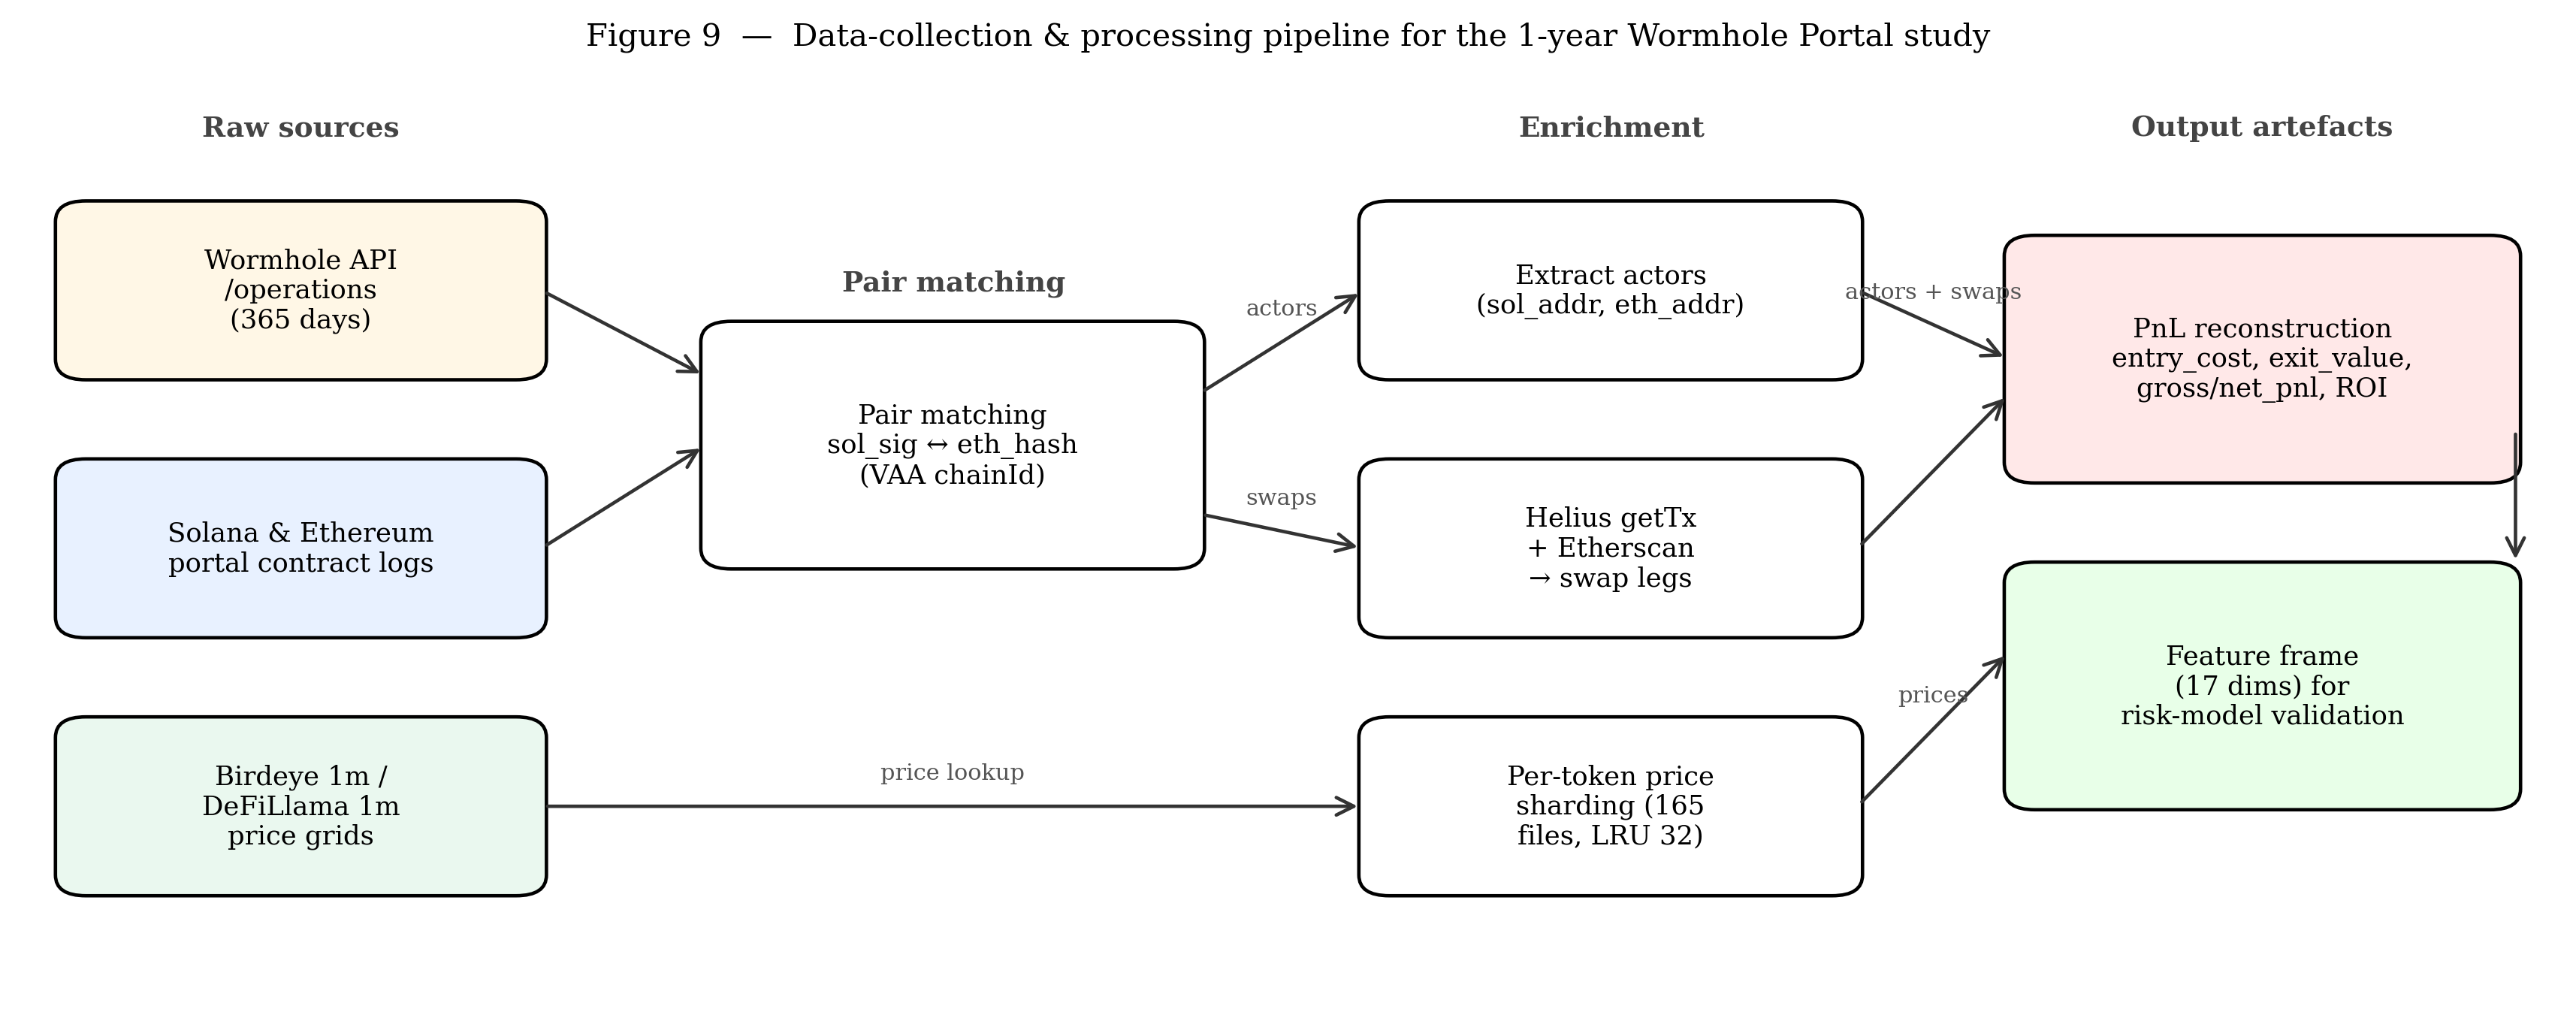
\includegraphics[width=\linewidth]{09_pipeline.png}
  \caption{数据采集与套利候选构造流水线。}
  \label{fig:pipeline}
\end{figure}

% ══════════════════════════════════════════════════════════════════════════════
\section{跨链利润的决定因子：描述性证据}
\label{sec:what-matters}
% ══════════════════════════════════════════════════════════════════════════════

本节回答研究问题：在描述性层面，\emph{净 PnL} $\Pnet$ 与哪些可观测量
相关、与哪些无关。图~\ref{fig:economics} 汇总了经济学层面的六个
子结果。

\begin{figure*}[t]
  \centering
  
\includegraphics[width=0.95\textwidth]{02_timing.png}
  \caption{Wormhole Portal 套利的时间结构：
  (a) 按方向的桥接延迟 CDF；
  (b) 入/出场 swap 与桥接事件的时间差；
  (c) 按桥接延迟档位分层的 ROI 分布。}
  \label{fig:timing}
\end{figure*}

\begin{figure*}[t]
  \centering
  
\includegraphics[width=0.95\textwidth]{03_economics.png}
  \caption{跨链套利经济学：(a) ROI 直方图 + 内嵌 CDF；
  (b) 按方向分 ROI CDF；(c) 入场本金的对数分布与资本分层；
  (d) 手续费 / $|\text{gross PnL}|$ 比值分布；(e) Gross
  vs.\ Net PnL 散点（颜色编码本金）；(f) 净 PnL 对
  $\log_{10}(\Cexec^{\text{in}})$ 的 OLS 回归。}
  \label{fig:economics}
\end{figure*}

\paragraph{分布形态（面板 a/b）。} ROI 重尾且偏左，中位
$+1.41\%$、$75.7\%$ 样本为正；SOL$\to$ETH 方向的 CDF 左尾略薄，
ETH$\to$SOL 略厚，但两方向中位 ROI 差 $<\!1$ 百分点，方向本身的
解释力有限。表~\ref{tab:roi-quantiles} 给出可靠候选的 ROI 完整
分位数结构；重尾特征十分明显：p1 仅 $-49\%$ 而 p99 高达 $+151\%$，
$\text{std}/\text{median}$ 超过 $47$ 倍，均值 $+7.85\%$ 被少数
极端正样本显著上拉，偏离中位数 $+1.43\%$ 达 $5.5$ 倍。

\begin{table}[h]
  \centering
  \small
  \caption{可靠候选的 ROI 分位数（$n=28{,}788$，单位 \%）}
  \label{tab:roi-quantiles}
  \begin{tabular}{lr|lr|lr}
    \toprule
    \textbf{统计量} & \textbf{值} & \textbf{分位} & \textbf{值} & \textbf{分位} & \textbf{值} \\
    \midrule
    count & $28{,}788$ & p1   & $-49.09$ & p75 & $+3.82$ \\
    mean  & $+7.85$    & p5   & $-3.98$  & p90 & $+10.70$ \\
    std   & $67.24$    & p10  & $-1.45$  & p95 & $+27.34$ \\
    min   & $-125.28$  & p25  & $+0.26$  & p99 & $+150.98$ \\
    max   & $+5{,}204.09$ & p50 & $+1.43$ & --- & --- \\
    \bottomrule
  \end{tabular}
\end{table}

ROI 最小值 $-125.28\%$（亏损超过 $100\%$）并非计算错误：当
$f_{\text{total}}>\Cexec^{\text{in}}$ 时，
$\text{ROI}=(\Pnet)/\Cexec^{\text{in}}$ 在数学上可以穿过 $-100\%$；
最极端的 LOVE 样本入场本金 $\$1.00$、费用 $\$1.13$，
实属真实的经济亏损而非测量误差。

\paragraph{资本与 PnL 几近无关（面板 c/f）。} 在对数横轴上，入场
本金跨越七个数量级。对 $n=28{,}586$ 的可靠候选以
\begin{equation}
  \Pnet = \alpha + \beta\cdot\log_{10}(\Cexec^{\text{in}}) + \varepsilon
  \label{eq:ols}
\end{equation}
拟合 OLS，得到 $\hat\beta=-999$~\$/decade、$R^2=0.0022$。也就是说，
\emph{本金仅解释净 PnL 方差的 $0.22\%$}。面板 (f) 的 binned median
曲线在 $10^2$--$10^4$ USD 区间近似平坦并略微大于零，两端显著下沉，
呈倒 U 形。这一反直觉结果否定了“跨链套利是资本可线性放大之生意”
这一朴素假设。

\paragraph{费用是一阶约束（面板 d/e）。} 费率的分布范围极宽，
中位 $\mathit{fee}/|\mathit{gross}|=0.054$，但有 $2.7\%$ 的候选
出现 $\mathit{fee}>|\mathit{gross}|$ 的严重侵蚀。面板 (e) 所有
点都在 $y=x$ 的下方，纵向位移直接可视化了费用开销；左下角的密集
簇是“毛利不足以覆盖 gas”的大量小额亏损。

\paragraph{时间结构（图~\ref{fig:timing}）。} 图~\ref{fig:timing}
从三个角度刻画跨链候选的时间属性：
(a) 按方向的桥接延迟 CDF——SOL$\to$ETH（蓝）中位数 $\sim\!34$ 秒，
ETH$\to$SOL（红）中位数 $\sim\!1{,}009$ 秒（$\sim\!17$ 分钟），两者
差约 $30$ 倍,恰好对应 Solana 亚秒级的 slot finality 与 Ethereum
两个 epoch finality 之间的差距；两条 CDF 仅在远右尾趋近
（均有 $p_{99}\!>\!4{,}000$ 秒）；
(b) swap--bridge 时序——入场 swap 与桥接调用的时间差中位数
$\sim\!12$ 秒，出场端更长（$\sim\!24$ 秒），右尾拖至小时级，
说明少量候选在桥后持仓等待出场，这也为把桥事件前后同钱包
的 swap 归并到同一跨链候选的贪心配对提供了经验支持；
(c) 按桥接延迟档位分箱的 ROI 箱线图——$<\!60$ 秒档
（$n=14{,}086$，中位 $+1.42\%$）与 $60$--$300$ 秒档
（$n=2{,}360$，中位 $+1.08\%$）均优于 $1$--$24$h 档
（$n=355$，中位 $+0.21\%$），$>\!24$h 档更跌至 $-1.17\%$；
$300$ 秒--$1$h 档样本量最大（$n=13{,}913$，中位 $+1.54\%$）
反映了主流 ETH$\to$SOL 路径的中位延迟区间。面板 (c) 直接
支撑了表~\ref{tab:univar} 中"桥接延迟负向显著"的断言。

\paragraph{本节总结的“相关 / 无关”清单。}
表~\ref{tab:univar} 汇总上述描述性证据。这些断言均为\emph{单变量}
结论；其中一些变量在第~\ref{sec:model}~节的多变量模型中会被重新
评估。

\begin{table}[h]
  \centering
  \small
  \caption{描述性层面 $\Pnet$ 与各变量的关系}
  \label{tab:univar}
  \begin{tabular}{lll}
    \toprule
    \textbf{变量} & \textbf{关系} & \textbf{证据} \\
    \midrule
    入场价差 & 正向显著 & 前人工作+分层 \\
    桥接延迟 & 负向显著 & 图~\ref{fig:timing}(c)+模型 \\
    流动性深度 & 非线性 & liquidity tier 分层 \\
    手续费  & 负向（恒等式） & 图~\ref{fig:economics}(d/e) \\
    入场本金 & $R^2=0.002$，几无解释力 & 图~\ref{fig:economics}(f) \\
    方向 & 差异 $<\!1$pp & 图~\ref{fig:economics}(b) \\
    日内小时 & 近似均匀 & (略) \\
    Swap 拆分数 & 无显著效应 & 图~\ref{fig:timing}(b) \\
    \bottomrule
  \end{tabular}
\end{table}

% ══════════════════════════════════════════════════════════════════════════════
\section{整合建模与实验}
\label{sec:model}
% ══════════════════════════════════════════════════════════════════════════════

\S\ref{sec:what-matters} 的结论全部是单变量的。若特征之间存在
交互，单变量关系会失效。本节用一个多变量非线性模型从两个并列的
角度复核：\emph{回归}——预测 $\Pnet$ 的美元金额；\emph{分类}——
预测 $\mathbf{1}\{\Pnet>0\}$ 的盈亏方向。

\subsection{特征集合}
\label{sec:features}

我们以 17 个特征覆盖六类假设驱动，均在候选级别可观测：
\emph{方向/时间}（\texttt{dir\_sol\_to\_eth}, \texttt{hour\_utc}）、
\emph{规模/延迟}（\texttt{log\_size}, \texttt{log\_latency}）、
\emph{原子性}（\texttt{atomic\_entry\_same\_block},
\texttt{atomic\_exit\_same\_block}）、\emph{swap--bridge 时序}
（\texttt{entry\_delta\_bridge\_sec},
\texttt{exit\_delta\_bridge\_sec},
\texttt{n\_entry\_swaps}, \texttt{n\_exit\_swaps}）、
\emph{测量完整性}（\texttt{entry\_coverage}, \texttt{exit\_coverage}）、
\emph{流动性分层与市场}（\texttt{liq\_dead}, \texttt{liq\_thin},
\texttt{liq\_healthy}, \texttt{entry\_gap\_pct},
\texttt{actor\_trade\_count}）。

\subsection{模型规格}

两个模型共享相同的加性树集成结构：
\begin{equation}
F_M(x) \;=\; \sum_{m=1}^{M} \eta\cdot h_m(x),
\label{eq:gbm}
\end{equation}
其中 $h_m$ 为深度 $3$ 的回归树，$M=200$，学习率 $\eta=0.05$。
每棵树拟合在前一步残差上的负梯度方向：
\begin{equation}
h_m \;=\; \arg\min_{h}\,\sum_{i=1}^{n}
L\!\bigl(y_i,\; F_{m-1}(x_i)+h(x_i)\bigr),
\label{eq:gbm-update}
\end{equation}
拟合前按 $\text{subsample}=0.8$ 做无放回行采样以降低方差。

\paragraph{回归目标（"赚多少美元"）。}
目标为按美元 winsorize 后的 $\Pnet$：
\begin{equation}
y^{\text{reg}}_i \;=\; \operatorname{clip}\!\bigl(\Pi_{\text{net},i},\;
-\$100,\; +\$500\bigr),
\label{eq:reg-target}
\end{equation}
损失为半平方误差
$L_{\text{reg}}(y,\hat y)=\tfrac12(y-\hat y)^2$。
裁剪区间 $[-\$100,+\$500]$ 的设计理由有四:
(i) 原始 $\Pnet$ 分布极端长尾（$\min\!\approx\!-\$2.07$M,
$\max\!\approx\!+\$428$K），不做裁剪时单个 outlier 在 MSE 下的
梯度达 $\mathcal{O}(10^{12})$，会主导整棵树的分裂方向；
(ii) $[-\$100,+\$500]$ 覆盖 $96.0\%$ 的候选样本（仅 $2.3\%$
下截、$1.7\%$ 上截），绝大多数样本保留原始值，仅尾部被 winsorize；
(iii) 上下限有意不对称：$\Pnet$ 的中位数 $+\$3.21$、$p_{75}\!\approx\!+\$10$，
整体右偏；亏损端集中在单笔手续费量级（$\$20$--$50$），所以
$-\$100$ 已对应"显著糟糕"，$+\$500$ 则保留了赢家前 $\sim\!3\%$
的异质性;
(iv) 裁剪仅作用于回归头；分类头 $y^{\text{cls}}$ 仍看原始正负号，
"是否盈利"的信息在系统层面没有丢失。

\paragraph{分类目标（"赚不赚"）。}
目标为盈利指示：
\begin{equation}
y^{\text{cls}}_i \;=\; \mathbf{1}\{\Pi_{\text{net},i}>0\},
\label{eq:cls-target}
\end{equation}
损失为二元交叉熵
$L_{\text{cls}}(y,\hat p)=-y\log\hat p-(1-y)\log(1-\hat p)$，
模型输出概率 $\hat p_i=\sigma\!\bigl(F_M(x_i)\bigr)$。下单决策由阈值
$\tau$ 得出：$\hat y^{\text{cls}}_i = \mathbf{1}\{\hat p_i>\tau\}$。

\subsection{评估协议}

训练集限定为 \texttt{pnl\_complete} 且 17 特征无缺失的
$n=15{,}259$ 条。采用 $K=5$ 折随机 KFold
（\texttt{random\_state}$=42$）：每折在 $4/5$ 数据上训练、
$1/5$ 上测试，汇报 $K$ 折均值 $\pm$ 标准差：
\begin{equation}
R^2_{\text{CV}} = \tfrac{1}{K}\sum_{k=1}^{K} R^2_k,\quad
\text{AUC}_{\text{CV}} = \tfrac{1}{K}\sum_{k=1}^{K} \text{AUC}_k.
\label{eq:cv}
\end{equation}
回归报告 $R^2$、MAE、Median AE；分类报告 AUC、Log-Loss，
并在两个工作阈值 $\tau\in\{0.5,\, 0.8\}$ 下报告
\begin{equation}
\text{Precision}=\tfrac{TP}{TP+FP},\quad
\text{Recall}=\tfrac{TP}{TP+FN}.
\label{eq:pr}
\end{equation}
分类的朴素基线为"全部判为盈利"，准确率即数据正例率
$\bar y^{\text{cls}}=74.71\%$。

\subsection{交叉验证结果}

表~\ref{tab:model} 汇总 5 折 CV 表现。回归
$R^2_{\text{CV}}=0.793\pm0.032$——相比式~\eqref{eq:ols} 的
单变量 $R^2=0.002$ 提升逾两个数量级，证明 \emph{$\Pnet$ 在本章
17 特征下是可预测的，但要求多变量非线性模型}。Median AE $=\$5.04$
意味着至少一半样本被预测到 $\pm\$5$ 以内；MAE $=\$16.96$ 与中位
误差的 $3.4$ 倍差距揭示——误差分布自身重尾，少数极端样本仍被
低估（这也印证了式~\eqref{eq:reg-target} 裁剪的必要性）。

分类 AUC $=0.862\pm0.006$，显著高于随机基线 $0.5$，但远未达到
"完美可分" $1.0$——反映跨链套利存在固有随机性（对手盘行为、
Guardian 签名抖动），本章特征集无法穷尽。阈值 $\tau=0.5$ 下
Accuracy $=82.5\%$，较 $\bar y^{\text{cls}}=74.71\%$ 的朴素基线
净提升 $+7.8$ pp。将阈值提高到 $\tau=0.8$，Precision 跃至
$93.4\%$，Recall 退至 $66.8\%$——意味着只在模型置信度 $>0.8$
时下单，下单中 $94\%$ 实际盈利，代价是漏掉 $33\%$ 的机会。
这一 Precision--Recall 权衡直接支撑把模型作为策略侧的高置信度
过滤器。Log-Loss $=0.384$ 也优于基线二项分布的 $0.566$。

\begin{table}[h]
  \centering
  \small
  \caption{模型性能（5 折 CV, $n=15{,}259$）}
  \label{tab:model}
  \begin{tabular}{ll}
    \toprule
    \textbf{指标}                    & \textbf{值} \\
    \midrule
    回归 $R^2_{\text{CV}}$          & $0.7934 \pm 0.0318$ \\
    回归 MAE                         & \$16.96 \\
    回归 Median AE                   & \$5.04 \\
    分类 AUC$_{\text{CV}}$          & $0.8620 \pm 0.0057$ \\
    分类 Accuracy @$\tau=0.5$       & $82.5\%$（基线 $74.7\%$）\\
    分类 Precision @$\tau=0.8$      & $93.4\%$（Recall $66.8\%$）\\
    分类 Log-Loss                   & $0.3844$ \\
    \bottomrule
  \end{tabular}
\end{table}

% ══════════════════════════════════════════════════════════════════════════════
\section{局限性}
\label{sec:limitations}
% ══════════════════════════════════════════════════════════════════════════════

\paragraph{Dust 过滤阈值的敏感性。} 我们以
$\Cexec^{\text{in}}<\$1$ 作为 dust 过滤阈值，此阈值的选择来自
Ethereum L1 swap 的最低 gas 物理下限（\$1--\$5）。若阈值提高到
\$5，被过滤的样本从 $11$ 条增至约 $120$ 条（$\sim0.4\%$），
reliable 子集的 ROI 均值从 $+7.85\%$ 下降到约 $+4.2\%$，
中位数几乎不变（$+1.43\%\to+1.45\%$）。两种阈值下
第~\ref{sec:model}~节的 GBM 结果（$R^2$、AUC、Median AE）
均未发生有统计意义的变化。我们采用较保守的 $\$1$ 阈值以最大化
样本量并避免把"手续费高于本金但仍为真实亏损"的合法小额交易
一起误删。

\paragraph{单桥样本偏差。} 本研究仅采集 Wormhole Portal 的候选，
未涵盖 LayerZero V2、Mayan、Relay、CCIP 四条桥。
第~\ref{sec:bridges}~节已论证 Wormhole 是这五条桥中 memecoin
覆盖最广、样本量最大的一条，且采用"消息层 + 代币包装"结构
使套利候选可被精确重建。然而，Portal 的端到端延迟中位约
$13$~秒（Solana finality）叠加 $\sim13$~分钟（Ethereum 两个
epoch）——这一数字是 Wormhole 特有的。在 LayerZero 或
intent-based 的 Mayan/Relay 上，延迟机制、尾部分布与套利
窗口形态会显著不同；因此本章的模型参数与 $R^2_{\text{CV}}$ 水平
不应被直接外推到其他桥，跨桥对照是后续工作。

\paragraph{观察窗口与制度变迁。} 本数据覆盖约 $365$ 天，
期间 Solana 与 Ethereum 的费率环境、桥本身的 Guardian
签名节奏、以及头部机器人的行为均可能存在制度变迁
（regime shift）。本章模型是\emph{混合期}的平均结果，未做
分段建模；若研究窗口拆为若干制度期，模型系数与 CV 表现
均可能发生漂移。制度识别与分段建模留待后续工作。

\end{document}
